% !Mode:: "TeX:UTF-8"
% !TEX program  = xelatex
% !BIB program  = biber
\documentclass[AutoFakeBold,AutoFakeSlant,language=english,degree=bachelor]{sustechthesis}
% 1. AutoFakeBold 与 AutoFakeSlant 为伪粗与伪斜,如果本机上有相应粗体与斜体字体,请使用 xeCJK 宏包进行设置,例如:
%   \setCJKmainfont[
%     UprightFont = * Light,
%     BoldFont = * Bold,
%     ItalicFont = Kaiti SC,
%     BoldItalicFont = Kaiti SC Bold,
%   ]{Songti SC}
%
% 2. language=chinese 基于为 ctexart 文类提供的中文排版方案修改,如果使用英文进行论文创作,请使用 language=english 选项。
%
% 3. degree=bachelor 为 sustechthesis 文类提供的本科生毕业论文模板,其他可选项为 master 与 doctor,但是均未实现,如果您对此有兴趣,欢迎 PR。
%
% 4. sustechthesis.cls 文类主要参考自去年完成使命的 sustechthesis.tex,在这一年的时间,作者的 TeX 风格与常用宏包发生许多变化,因为之前的思想为仅提供必要的格式修改相关代码,所以转换为文类形式所进行的修改较少,而近期的风格与常用宏包均体现在以下的例子文件中。
%
% 5. 示例文件均放置于相应目录的 examples 文件夹下,构建自己论文时可暂时保留,用以检索接口与使用方法。
%
% 6. 英文目录需要居中可以使用:\renewcommand{\contentsname}{\centerline{Content}}
%
% 7. LaTeX 中公式编号括号样式及章节关联的方法:https://liam.page/2013/08/23/LaTeX-Formula-Number/

\input{config/preamble.tex} % 导言区
% !Mode:: "TeX:UTF-8"
% !TEX program  = xelatex
\设置信息{
    % 键 = {{中文值}, {英文值}},
    分类号 = {{}, {}},
    编号 = {{}, {}},
    UDC = {{}, {}},
    密级 = {{}, {}},
    % 仅题目(不含副标题)、系别、专业,支持手动 \\ 换行,不支持自动换行。
    题目 = {{基于单目测距与离轴透视投影的裸眼3D\\效果实现}, {Naked-Eye 3D Implementation \\ Based on Monocular Distance Measurement \\ and Off-axis Perspective Projection}},
    % 如无需副标题,删除值内容即可,不可删除键定义。
    副标题 = {{}, {}},
    姓名 = {{黄梓通}, {Zitong Huang}},
    学号 = {{12012710}, {12012710}},
    系别 = {{计算机科学与工程系}, {Computer Science and Engineering}},
    专业 = {{计算机科学与技术}, {Computer Science and Technology}},
    指导老师 = {{宋轩}, {Xuan Song}},
    时间 = {{2024年6月7日}, {Jun 7, 2024}},
    职称 = {{副教授}, {Associate Professor}},
}
 % 论文信息
\begin{document}

% \中文标题页
\英文标题页

% \中文诚信承诺书
\英文诚信承诺书

\前序格式化
\摘要标题
% !Mode:: "TeX:UTF-8"
% !TEX program  = xelatex

\begin{英文摘要}{VR, Head-Track, Off-axis Projection, Kalman Filter, OpenCV, Unity}

% Immersive virtual reality (VR) systems have demonstrated considerable potential across a spectrum of applications ranging from entertainment to education. Existing VR solutions typically necessitate the use of specialized headgear, thereby limiting their accessibility and convenience.

Immersive 3D systems have demonstrated considerable potential across a spectrum of applications ranging from entertainment to education. Existing 3D solutions typically necessitate the use of specialized glasses and professional photographic devices, thereby limiting their accessibility and convenience. In this work, we introduce an innovative 3D system that employs monocular ranging and off-axis projection techniques to facilitate an immersive experience without the encumbrance of cumbersome equipment. Our system dynamically adjusts the virtual scene based on the viewer's position, thereby providing a "window" into the virtual world that mimics the real-world illusion.

To achieve this objective, we propose a lightweight and cost-effective head tracking solution that leverages YuNet facial keypoint detection, integrated with the Enhanced Perspective-n-Point (ePnP) algorithm and Kalman filtering, to realize effective monocular head tracking. Furthermore, the study introduces a novel algorithm for optimizing image display on curved screens. This algorithm involves the horizontal segmentation of images and adapts each segment to the curvature, optimizing the image presentation on curved screens. This method ensures that the displayed images maintain their intended appearance, thereby enhancing the realism of the 3D experience. Our approach has been fine-tuned with a combination of real-time computational models and mobile-friendly implementations to ensure efficiency and responsiveness.

% This technology's ingenuity lies in its ability to surmount both the physical and fiscal impediments associated with standard VR modalities, while also facilitating a more organic and intuitive user interaction by meticulously tracking the user’s facial and eye movements. The prospective applications of this methodology are extensive, spanning entertainment and gaming to sectors like education, healthcare, and industrial design, offering an immersive digital milieu accessible without the dependency on supplementary apparatus.
\end{英文摘要}

\begin{中文摘要}{VR, Head-Track, Off-axis Projection, Kalman Filter, OpenCV, Unity}

% 在虚拟现实(VR)领域,实现真正沉浸式体验通常需要使用笨重的头戴设备,这会影响用户的舒适度和可及性。本项目引入了一种新颖的VR系统,旨在通过单目测距和偏轴投影技术规避这些限制。该系统将标准显示屏转变为通向虚拟环境的动态“窗口”,根据观众的位置调整视觉输出。这种调整模拟了现实世界中的视角变化,在无需专用设备的情况下增强了虚拟体验的真实性。我们详细介绍了该技术的开发,强调其轻量化实现和广泛应用的潜力,从娱乐到教育培训等多个领域。初步评估显示,该系统在提供引人入胜和互动的用户体验方面效果显著,表明其作为传统VR解决方案的实际替代方案的可行性。


沉浸式3D系统在娱乐和教育等广泛应用领域展现出巨大的潜力。现有的3D解决方案通常需要使用专业的摄影设备和特制眼镜,从而限制了其普及性和便利性。在本研究中,我们引入了一种创新的3D系统,该系统采用单目测距和偏轴投影技术,无需笨重设备即可提供沉浸式体验。我们的系统能够根据观众的位置动态调整虚拟场景,从而提供一个“窗口”式的虚拟世界,模拟现实世界的错觉。

为了实现这一目标,我们提出了一种轻量且成本效益高的头部追踪解决方案,该方案利用YuNet面部关键点检测,与增强型透视n点(ePnP)算法和卡尔曼滤波集成,实现有效的单目头部追踪。此外,本研究还引入了一种优化曲面屏幕图像显示的新算法。该算法通过对图像进行水平分割,并根据曲率调整每个分段,从而优化图像在曲面屏幕上的显示效果。此方法确保显示的图像保持其预期外观,从而增强3D体验的真实感。我们的方法结合了实时计算模型和移动设备友好的实现,确保了效率和响应能力。


\end{中文摘要}
 % 论文摘要

\目录\clearpage % 目录及换页

\正文格式化
\part{Introduction}

\section {Introduction}

% task 
% traditional method
% current method
% lack of current method
% main update of your method
% additional output

3D Display System aims to proide immersive and interactive experiences of virtual scenarios base on human vision illusions. Since the concept of metaverse is introduced by Facebook, 3D display technology is attracting more and more attetion from both academic and industrial field.

While earlier 3D display base on binocular vision by allying two images as binocular disparity, the traditional 3D display system usually requires professional photographic capture devices and specialized glasses, which limits the accessibility and convenience of the system. Recent years naked-eye display systems based on horizontal parallax coms into public view. L-shaped monitor on Taiguli Chengdu(Figure 1a) is a typical example of horizontal parallax illusion applications, since the shape provide additional depth illusion.\cite{Wang2024} Althought the L-shaped display system excuse users from wearing heavy glasses, the expensive price and fixed position of the viewer still limit its accessibility and convenience.

\begin{figure}[htb]
    \centering
    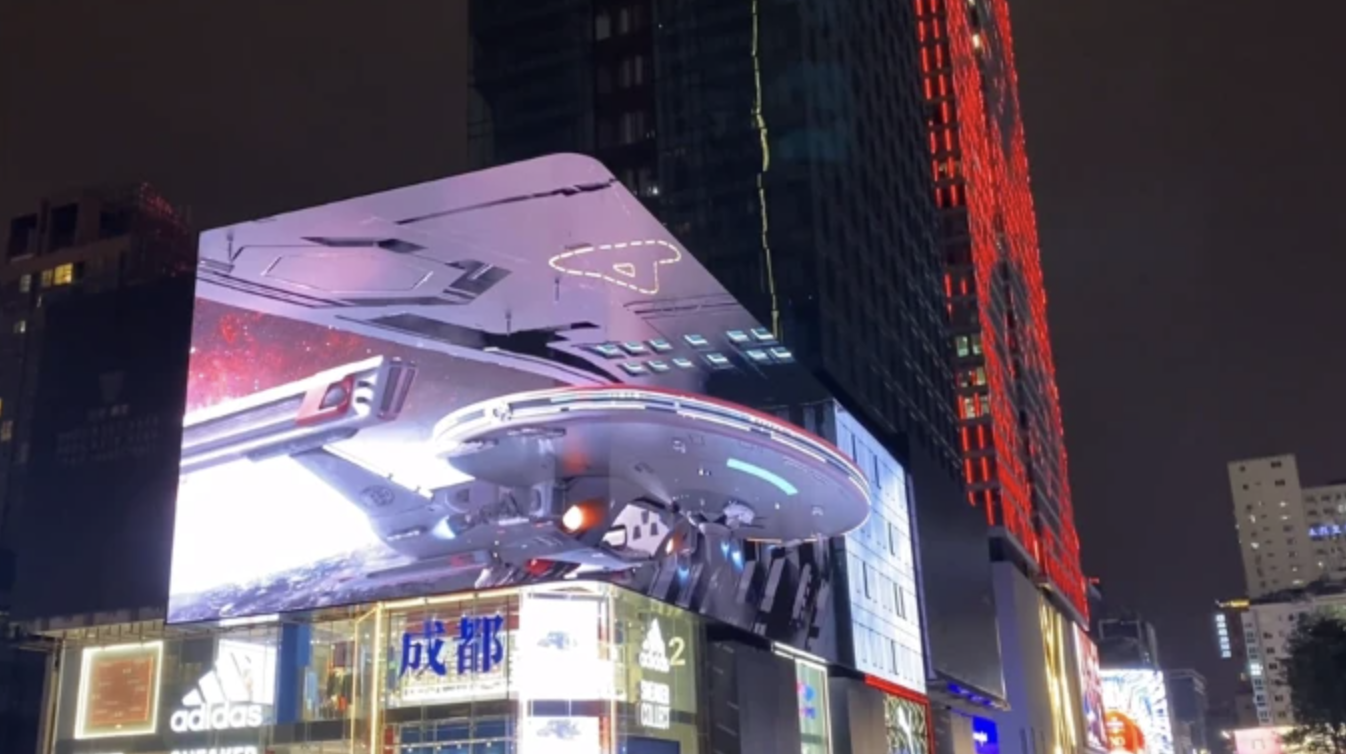
\includegraphics[width=0.7\textwidth]{figures/L-shaped.png}
    \caption{L-shaped Display Monitor}\label{F:test-a}
\end{figure}

To tackle these problems, another motion parallax based light-weight solution is proposed\cite{ALLISON20031879}. Wang\cite{Wang_2018} introduce a 3D display system based on Kinect SDK, and Peder. 2019 \cite{TheParallaxView} developed an IOS application based on iPhoneX's TrueDepth camera(Figure 1b). These two systems both use the combination of head-track and off-axis perspective projection, provided a customer-oriented 3D display system. Compare with L-shaped solutions, motion-based 3D display system is more flexible and cheaper, since it only requires a camera and a display device.

\begin{figure}[htb]
    \centering
    \includegraphics[width=0.6\textwidth]{example-image-a}
    \caption{Horizontal Parallax}\label{F:test-a}
\end{figure}

However, the head-track part in these two systems is essentially using SDK procided by hardware manufacturers(Kinect in Wang's work, and iPhone in Pader's work), which suffers from hardward limitations. Although depth measurement devices exactly provides a more convenience and stable solution, the flexibility and expensibility cannot reach requirements. Consider a general head-track task which need to inference human head's position, given a specific usage scenary, a head-track task requirement usually need to cover difference specific conditions. For example, laptop deployments without an external depth camera or laser radar. Also, SDK-based traking solutions is not flexible enough to handle possible bugs and errors, since the source code is not open to the public, makes it's harder to be mentained by single developer. In additional, SDK-based solution can only be deployed as assemblyies or on specific devices: the former needs extra cost for expensive professional devices, and the latter limits the system's application for different users, which introduce extra cost and limit naked 3d systems' further application.

\begin{figure}[htb]
    \centering
    \includegraphics[width=0.5\textwidth]{example-image-a}
    \caption{Head Track Working Flow. }\label{F:test-a}
\end{figure}

This work proposed a new head-track solution based on monocular distance measurement and off-axis projection, privide a cheaper and more flexible solution for 3D display system. As shown in figure 2, this work can inference human head's position with a single camera with the support of face landmark detection algotithm and researches of perspective-n-point(PnP) problem, without surpports of depth measurement hardwares. The main update of this work is the combination of face landmark detection and ePnP algorithm\cite{EPnP_2009}, which provide a more flexible and cheaper solution for 3D display system. 

\begin{figure}[htb]
    \centering
    \includegraphics[width=0.5\textwidth]{example-image-a}
    \caption{Image correction}\label{F:test-a}
\end{figure}

Beside monocular head-tracking, display optimization is also considered as an important of vision illusions. Since most of motion parallax based 3d systems only consider standard display monitors, we proposed a noval correction algorithm for curved displays. By accepting result from head-traking algorithms, correction algorithm can adjust displayed frames to fit the view angle of users, which is more appropriate for curved displays which is more and more popular in recent years.

The contributions of this work include:

\begin{itemize}
    \item A new head-track system based on monocular distaance measurement, which provide a cheaper and more flexible solution for 3D display system compared with depth-camera based methods.
    \item A correction algorithm for curved displays, which is more appropriate for curved displays which is more and more popular in recent years.
\end{itemize}

In conclusion, this work provides a new head-track system based on monocular distaance measurement, which is more flexible and cheaper than traditional depth-camera based methods. Conbined with off-axis perspective projection and the correction algorithm for curved displays, this work provides a more flexible and cheaper solution for 3D display system.


\section {Related Work}

\subsection {Motion Parallax}

Motion parallax is a visual illusion that occurs when objects at different distances move across the observer's field of view. This phenomenon is a key depth cue in human vision, enabling the perception of depth and distance in the absence of stereoscopic vision. Principles of motion parallax can provide depth information to human brain's neural is the comparation of motion speed of different objects in the same view. e.g., when a person moves his head, objects closer to the observer appear to move faster than objects further away, providing a sense of depth and distance. Hanes et al.(2008) explain the mathemetical details of motion parallax, providing geometry and experimental evidence of it\cite{Hanes2008}, shown as Fig.3.

\begin{figure}[htb]
    \centering
    \includegraphics[width=0.5\textwidth]{example-image-a}
    \caption{Motion parralax reminder: $d\theta / dt$ is a good cue for motion derectory, while $w(D, \theta)$ is velocity's\cite{Hanes2008}}\label{F:test-a}
\end{figure}

This effect is widely used in 3D display systems: Lee et al. (2019) designed a head-traking system based on Nintendo Wii remote, constructed a depth illusion with the application of motion parallax\cite{Lee}. Apple's IOS7 also introduced a light motion parallax effect. By move applications' icons lightly when users move their phone, Apple provides a more immersive and interactive experience for users.\cite{Apple2014}.
\subsection{Face  Landmark Detection}
From early techniques, face landmark is mainly implemented by statistical and simple machine learning methods. The \textbf{Active Shape Model (ASM)}, \textbf{Active Appearance Model (AAM)}, and \textbf{Constrained Local Model (CLM)} \cite{WANG201850} \cite{Khabarlak_2022} are foundational methods that employ statistical models to fit a deformable face mesh, optimized for controlled environments but underperforming in in-the-wild scenarios. Subsequent advancements, such as \textbf{Ensemble of Regression Trees (ERT)} \cite{Kazemi_2014_CVPR} employed by \textbf{dlib}, improved accuracy by using a cascade based on gradient boosting, making it highly efficient for real-time applications despite its limitations with pose variations.

\begin{figure}[htb]
    \centering
    \includegraphics[width=0.5\textwidth]{example-image-a}
    \caption{cascade based gradient boosting }\label{F:test-a}
\end{figure}

The evolution towards neural network-based approaches has introduced a diverse array of backbones, enhancing the detection capabilities under unconstrained conditions. Techniques such as the \textbf{Hourglass} \cite{Newell_2016_ECCV} and \textbf{HRNet} \cite{Sun_2019_CVPR} architectures leverage heatmap-based methods to improve landmark localization accuracy by predicting probabilistic heatmaps for each landmark . These methods are robust against pose variations and occlusions, crucial for applications requiring high fidelity in dynamic environments.
\textbf{Style Aggregated Network (SAN)}\cite{Dong_2018_CVPR} employs ResNet-152 \cite{He_2016_CVPR} to handle variability in image styles by stabilizing landmark detection across different photographic conditions, illustrating the importance of adaptive models in diverse real-world applications.

YOLO-series\cite{Redmon_2016_CVPR} are also considered as a efficient method in face landmark detection. As a one-stage object detection model, YOLO detect objects' position and classes by directly inference features extract by CNN model. Base on YOLO, Qi et al. (2022) developed \textbf{YOLO5Face}\cite{Qi2022YOLO5Face}, a face detector built upon the YOLOv5 object detection framework. The model incorporates modifications such as a landmark regression head and various optimizations for processing both large and small faces effectively. YOLO5Face is designed to provide robust face detection capabilities across different model sizes, catering to various application requirements from high-performance setups to real-time detection on mobile or embedded devices. The detector achieves state-of-the-art performance on the WiderFace dataset, demonstrating its efficiency and accuracy in diverse conditions. In following two years, YOLOv7-face\cite{YOLOv7Face} and YOLOv8-face\cite{YOLOv8Face} is developed, which further improve the performance of face detection and landmark detection.

\begin{figure}[htb]
    \centering
    \includegraphics[width=0.6\textwidth]{example-image-a}
    \caption{YOLOv1 structure}\label{F:test-a}
\end{figure}

In 2023, Wu et developed \textbf{YuNet}\cite{Wu_2023}, an advanced face detection model specifically engineered for edge computing devices, which emphasizes minimal model size and maximized computational efficiency. The architecture of YuNet incorporates a streamlined feature extraction backbone and a simplified pyramid feature fusion technique, tailored to meet the stringent performance requirements of mobile and embedded systems with limited processing capabilities. This model is distinguished by its ability to deliver high-speed performance with an exceptionally low parameter count, making it particularly well-suited for real-time applications where both speed and accuracy are critical, yet resources are constrained.


\subsection{Target Tracking}
During these decades, target traking problem has gains lots of attetion in academic and industrial firld due to the universality of application. With sensor information stream input, tracking algorithms estimate target's motion state, applicated them in next-timestamp's pose estimation. Target tracking algorithms can mainly be divided into three categories: \textbf{Batch Processing}, \textbf{Recursive} and \textbf{Optimization-Based}\cite{KumarMondal2021}. Batch Processing methods observe one time period operate one specific time period to estimate target's motion state, with common algorithms like MLE, PLS, GA and sequencial networks. A typical problem of Batch Processing latency issue and data requirement, since batch processing need to wait for all data to be collected before processing.\cite{KumarMondal2021}. 

Recursive-based methods, typically Sequential Bayesian filter, performance better in real-time tracking and unbiased estimates\cite{KumarMondal2021}. One powerfule variant of Sequential Bayesian filter is Kalman Filter, proposed by Rudolf E. Kálmán in 1960\cite{Kalman1960}, designed to estimate target's motion state with noisy sensor information. Kalman Filter is widely used in target tracking, pose estimation, and sensor fusion.
\begin{figure}[htb]
    \centering
    \includegraphics[width=0.6\textwidth]{example-image-a}
    \caption{Kalman Filter Working Flow}\label{F:test-a}
\end{figure}

Another category of target tracking is Optimization-Based methods, developed on the basis of loss functions of tracking methods.\cite{KumarMondal2021}. Optimization-Based methods are more flexible and can be applied in various tracking scenarios, with common algorithms like Particle Filter, Mean Shift, and Deep Learning-based methods. However, since loss-fucntions' optimization introduce extra complexity, Optimization-Based methods are usually more computational expensive than Recursive-based methods.

\nocite{Khabarlak_2022}




% \part{Related Works and Preliminaries}

\section {Related Work}

\subsection {Motion Parallax}

Motion parallax is a visual illusion that occurs when objects at different distances move across the observer's field of view. This phenomenon is a key depth cue in human vision, enabling the perception of depth and distance in the absence of stereoscopic vision. Principles of motion parallax can provide depth information to human brain's neural is the comparation of motion speed of different objects in the same view. e.g., when a person moves his head, objects closer to the observer appear to move faster than objects further away, providing a sense of depth and distance. Hanes et al.(2008) explain the mathemetical details of motion parallax, providing geometry and experimental evidence of it\cite{Hanes2008}, shown as Fig.3.

\begin{figure}[htb]
    \centering
    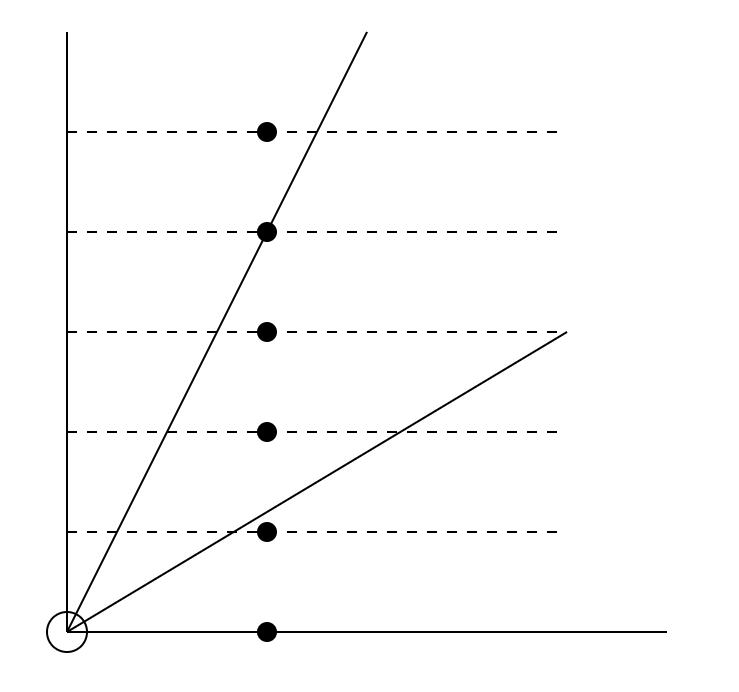
\includegraphics[width=0.5\textwidth]{figures/Introduction/motion.png}
    \caption{Motion parralax reminder: view angle difference is a good cue for motion derectory, while object's movement distance is velocity's\cite{Hanes2008}}\label{F:test-a}
\end{figure}

This effect is widely used in 3D display systems: Lee et al. (2019) designed a head-traking system based on Nintendo Wii remote, constructed a depth illusion with the application of motion parallax\cite{Lee}. Apple's IOS7 also introduced a light motion parallax effect. By move applications' icons lightly when users move their phone, Apple provides a more immersive and interactive experience for users.\cite{Apple2014}.
\subsection{Face  Landmark Detection}
From early techniques, face landmark is mainly implemented by statistical and simple machine learning methods. The \textbf{Active Shape Model (ASM)}, \textbf{Active Appearance Model (AAM)}, and \textbf{Constrained Local Model (CLM)} \cite{WANG201850} \cite{Khabarlak_2022} are foundational methods that employ statistical models to fit a deformable face mesh, optimized for controlled environments but underperforming in in-the-wild scenarios. Subsequent advancements, such as \textbf{Ensemble of Regression Trees (ERT)} \cite{Kazemi_2014_CVPR} employed by \textbf{dlib}, improved accuracy by using a cascade based on gradient boosting\cite{saberian2014boosting}, making it highly efficient for real-time applications despite its limitations with pose variations.

\begin{figure}[htb]
    \centering
    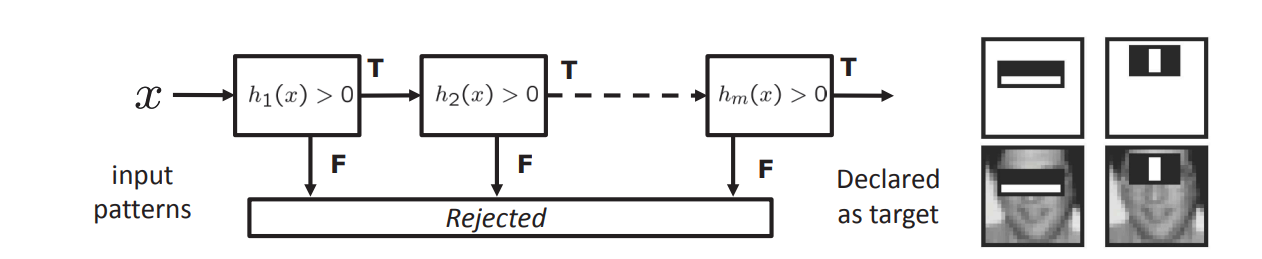
\includegraphics[width=1\textwidth]{figures/Introduction/cascade.png}
    \caption{Cascade based gradient boosting }\label{F:test-a}
\end{figure}

The evolution towards neural network-based approaches has introduced a diverse array of backbones, enhancing the detection capabilities under unconstrained conditions. Techniques such as the \textbf{Hourglass} \cite{Newell_2016_ECCV} and \textbf{HRNet} \cite{Sun_2019_CVPR} architectures leverage heatmap-based methods to improve landmark localization accuracy by predicting probabilistic heatmaps for each landmark . These methods are robust against pose variations and occlusions, crucial for applications requiring high fidelity in dynamic environments.
\textbf{Style Aggregated Network (SAN)}\cite{Dong_2018_CVPR} employs ResNet-152 \cite{He_2016_CVPR} to handle variability in image styles by stabilizing landmark detection across different photographic conditions, illustrating the importance of adaptive models in diverse real-world applications.

YOLO-series\cite{Redmon_2016_CVPR} are also considered as a efficient method in face landmark detection. As a one-stage object detection model, YOLO detect objects' position and classes by directly inference features extract by CNN model. Base on YOLO, Qi et al. (2022) developed \textbf{YOLO5Face}\cite{Qi2022YOLO5Face}, a face detector built upon the YOLOv5 object detection framework. The model incorporates modifications such as a landmark regression head and various optimizations for processing both large and small faces effectively. YOLO5Face is designed to provide robust face detection capabilities across different model sizes, catering to various application requirements from high-performance setups to real-time detection on mobile or embedded devices. The detector achieves state-of-the-art performance on the WiderFace dataset, demonstrating its efficiency and accuracy in diverse conditions. In following two years, YOLOv7-face\cite{YOLOv7Face} and YOLOv8-face\cite{YOLOv8Face} is developed, which further improve the performance of face detection and landmark detection.

% \begin{figure}[htb]
%     \centering
%     \includegraphics[width=0.6\textwidth]{example-image-a}
%     \caption{YOLOv1 structure}\label{F:test-a}
% \end{figure}

In 2023, Wu et developed \textbf{YuNet}\cite{Wu_2023}, an advanced face detection model specifically engineered for edge computing devices, which emphasizes minimal model size and maximized computational efficiency. The architecture of YuNet incorporates a streamlined feature extraction backbone and a simplified pyramid feature fusion technique, tailored to meet the stringent performance requirements of mobile and embedded systems with limited processing capabilities. This model is distinguished by its ability to deliver high-speed performance with an exceptionally low parameter count, making it particularly well-suited for real-time applications where both speed and accuracy are critical, yet resources are constrained.


\subsection{Target Tracking}
During these decades, target traking problem has gains lots of attetion in academic and industrial firld due to the universality of application. With sensor information stream input, tracking algorithms estimate target's motion state, applicated them in next-timestamp's pose estimation. Target tracking algorithms can mainly be divided into three categories: \textbf{Batch Processing}, \textbf{Recursive} and \textbf{Optimization-Based}\cite{KumarMondal2021}. Batch Processing methods observe one time period operate one specific time period to estimate target's motion state, with common algorithms like MLE, PLS, GA and sequencial networks. A typical problem of Batch Processing latency issue and data requirement, since batch processing need to wait for all data to be collected before processing.\cite{KumarMondal2021}. 

\begin{figure}[htb]
    \centering
    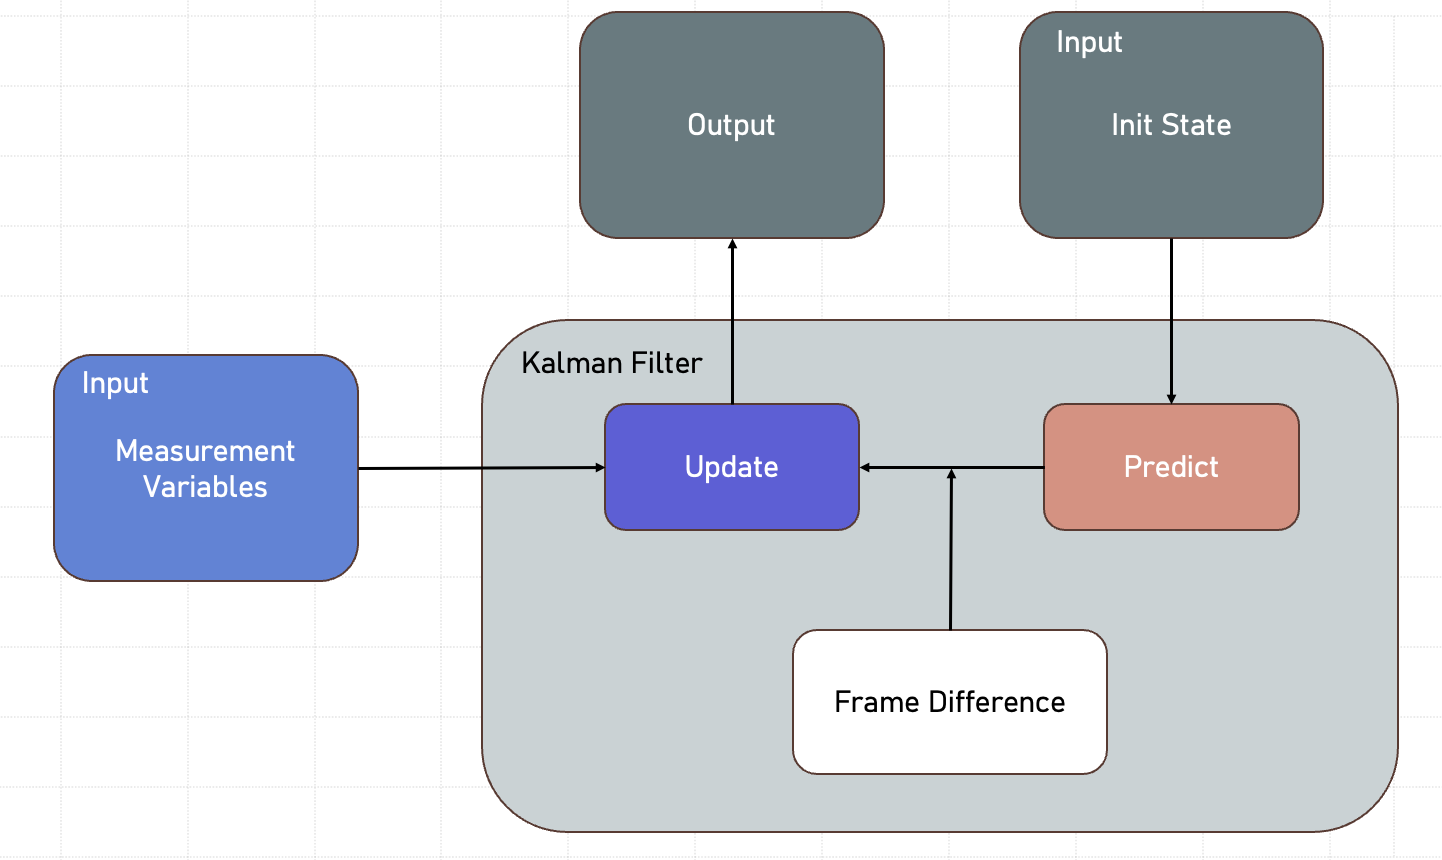
\includegraphics[width=1\textwidth]{figures/Introduction/KalmanFilter.png}
    \caption{Kalman filter working flow}\label{F:test-a}
\end{figure}

Recursive-based methods, typically Sequential Bayesian filter, performance better in real-time tracking and unbiased estimates\cite{KumarMondal2021}. One powerfule variant of Sequential Bayesian filter is Kalman Filter, proposed by Rudolf E. Kálmán in 1960\cite{Kalman1960}, designed to estimate target's motion state with noisy sensor information. Kalman Filter is widely used in target tracking, pose estimation, and sensor fusion.


Another category of target tracking is Optimization-Based methods, developed on the basis of loss functions of tracking methods.\cite{KumarMondal2021}. Optimization-Based methods are more flexible and can be applied in various tracking scenarios, with common algorithms like Particle Filter, Mean Shift, and Deep Learning-based methods. However, since loss-fucntions' optimization introduce extra complexity, Optimization-Based methods are usually more computational expensive than Recursive-based methods.

\nocite{Khabarlak_2022}

\section {Preliminaries}
This section introduces the basic concepts and technologies used in this project, including face landmark detection, Perspective-N-Point (PnP) problem, Kalman Filter, Perspective Projection and Off-axis Perspective Projection. We will introduce YuNet in section 3.1, and review the PnP problem in section 3.2. In section 3.3, we will introduce the Kalman Filter, including a simple derivation. In section 3.4, we will introduce the perspective projection and off-axis perspective projection, and explain why off-axis perspective projection is needed in our research.
\subsection{Face Landmark Detection}
Face landmark detection is one of the main tasks in computer vision. It is used to detect the key points of a face, such as the eyes, nose, and mouth. These key points can be used for various applications, such as face recognition, emotion detection, and head pose estimation. There are many different methods for face landmark detection, including traditional computer vision techniques and deep learning-based approaches. In this project, we will use a deep learning-based approach for face landmark detection, as YuNet provided in Sec2.2. OpenCV 4.5.4\cite{opencv_4_5_4} introduced YuNet in 2021 as one of face landmark detection API, which provide a fast and convinience way to complete face landmark detection task. In addition, a research compare YuNet a with traditional haar cascade detection in dlib, and YuNet performs better in both performance and accuracy. \cite{chen2022opencv}.

\subsection{Perspective-N-Point (PnP) Problem}
Perspective-N-Point (PnP) problem is a fundamental problem in computer vision, which is used to estimate the pose of a camera given a set of 3D points and their corresponding 2D projections. The PnP problem is commonly used in applications such as augmented reality, camera calibration, and robot localization. There are many different algorithms for solving the PnP problem, including the Direct Linear Transform (DLT) method, the Levenberg-Marquardt algorithm, and the RANSAC algorithm. 

\begin{figure}[htb]
    \centering
    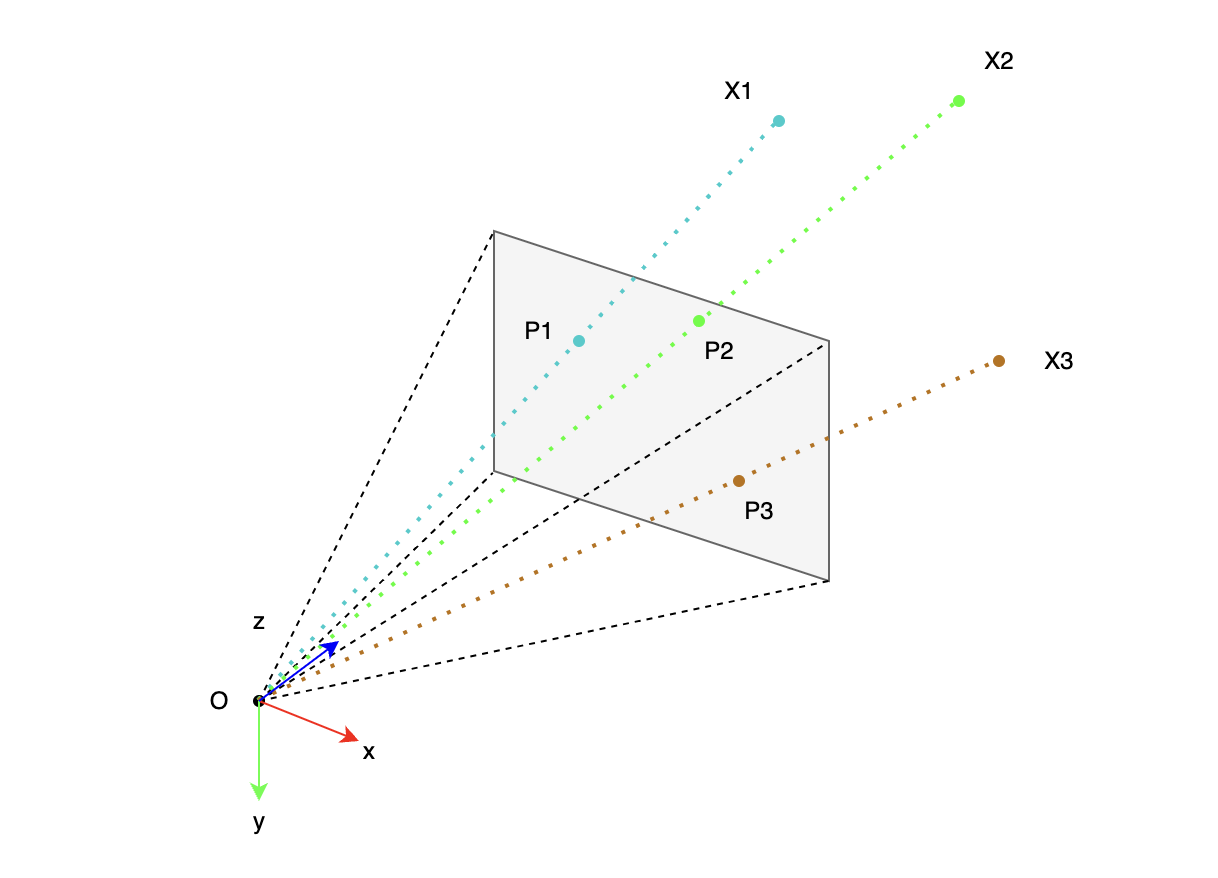
\includegraphics[width=1\textwidth]{figures/Introduction/PnP.png}
    \caption{Perspective-N-Point(PnP) problem}\label{F:test-a}
\end{figure}


\subsection{Kalman Filter}
Using face position provided by pnp solver directly usually is an effeient way, but not stable enough to cover noises from possible environments.  Since keypoints provided by detector is not stable enough to get a steady result, position solve by pnp-solver often meet unexpected oscillation and jittering. To solve the problem, we introduce kalman filter as a filter to smooth the movement of human head. 

Kalman Filter is a specific type of recursive Bayesian filter, which is used to estimate the state of a linear dynamic system from a series of noisy measurements. As a varietas of Bayesian filter, Kalman filter combain the prior knowledge of the system with the current measurement to provide an optimal estimate of the state of the system by a self-adjusting kalman gain $K$. 

The Kalman Filter is based on a linear dynamical system model, based on following elements:
\begin{itemize}
    \item State Vector $x_k$: State to be estimated of the  system.
    \item Measurement Vector $z_k$: Variable can be measured by sensors of the system. Note the measurement is noisy.
    \item State Transition Matrix $F_k$: State transition matrix, which describe the state transition of the system from prior state to current state.
    \item Measurement Matrix $H_k$: Measurement matrix, which describe the mapping from state space to measurement space.
    \item Process Noise Covariance Matrix $Q_k$: Covariance matrix of the process noise.
    \item Measurement Noise Covariance Matrix $R_k$: Covariance matrix of the measurement noise.
    \item Kalman Gain $K_k$: Gain of the Kalman filter, which is used to adjust the weight of the prior state and the measurement.
    \item State Covariance Matrix $P_k$: Covariance matrix of the prior state.
\end{itemize}

The Kalman Filter consists of two main steps: the prediction step and the update step. In the prediction step, filter predict the state of the system based on the prior state and the state transition matrix and update prior state covariance P:
\begin{equation}
    \hat{x}_{k|k-1} = F_k \hat{x}_{k-1|k-1} 
\end{equation}
\begin{equation}
    P_{k|k-1} = F_k P_{k-1|k-1} F_k^T + Q_k
\end{equation}


Once the measurement is available, the filter update the state of the system based on the measurement and the measurement matrix:
\begin{equation}
        K_k = P_{k|k-1} H_k^T (H_k P_{k|k-1} H_k^T + R_k)^{-1}
\end{equation}
\begin{equation}
        \hat{x}_{k|k} = \hat{x}_{k|k-1} + K_k(z_k - H_k \hat{x}_{k|k-1})
\end{equation}
\begin{equation}
        P_{k|k} = (I - K_k H_k) P_{k|k-1} 
\end{equation}

In update step, kalman gain is updated based on the measurement and the prior state covariance, and providing the optimal estimate of the state of the system in next step.

\subsection{Perspective Projection and Off-axis Perspective Projection}

Perspective projection is a common projection method in computer graphics and daily life. It is used to project a 3D point onto a 2D plane. Consider a 3d object point, perspective projection generated 2d coordinate by mapping it to a 2 * 2 * 2 rectangular-projection cube, where $x$ and $y$ are the 2D position and $z$ is the depth information of the 3D point.

As camera field of view($fov$) given, we can generate the perspective projection matrix as:

\[
\begin{bmatrix}
\frac{\cot \left( \frac{\text{fovy}}{2} \right)} {aspect} & 0 & 0 & 0 \\
0 & \cot \left( \frac{\text{fovy}}{2} \right) & 0 & 0 \\
0 & 0 & -\frac{f+n}{f-n} & -\frac{2fn}{f-n} \\
0 & 0 & -1 & 0
\end{bmatrix}
\]
Where $f$ is the far plane, $n$ is the near plane, and $aspect$ is the aspect ratio of the view plane. Fully explanation of perspective projection can be found in \cite{ahn_opengl_projection_matrix}.
    
\begin{figure}[htb]
    \centering
    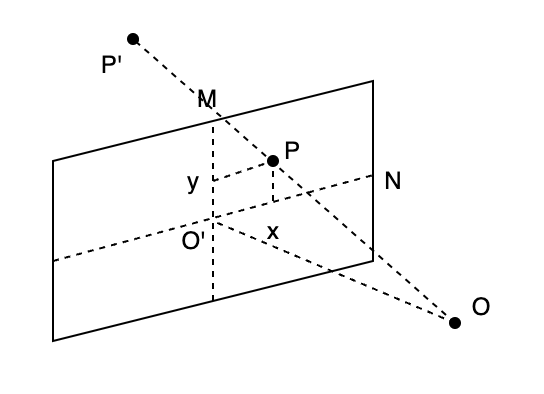
\includegraphics[width=0.7\textwidth]{figures/Preliminaries/pinCamera.png}
    \caption{Pinhole camera model, where $O$ is observer's position, $O'$ is view point, $O'MN $ is view plane, $P$ is the 2D projection on view plane of a 3D point, and $M$, $N$ is the orthogonal projection from the viewpoint to the upper/right boundary of the plane.}\label{F:test-a}
\end{figure}

% \begin{figure}[htb]
%     \centering
%     \begin{subfigure}[t]{.45\linewidth}
%         \centering
%         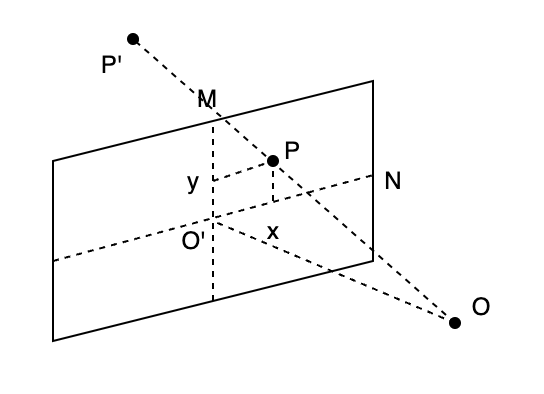
\includegraphics[width=1\textwidth]{figures/Preliminaries/pinCamera.png}
%         \caption{Pinhole camera model, where $O$ is observer's position, $O'$ is view point, $O'MN $ is view plane, $P$ is the 2D projection on view plane of a 3D point, and $M$, $N$ is the orthogonal projection from the viewpoint to the upper/right boundary of the plane.}\label{F:test-a}
%     \end{subfigure}
%     % \begin{subfigure}[t]{.45\linewidth}
%     %     \centering
%     %     \includegraphics[width=1\textwidth]{example-image-a}
%     %     \caption{The target of perspective project is mapping 3D points to a 2 * 2 * 2 cube, where x and y are the related 2D coordinate and z is the depth information of the 3D point.}\label{F:test-b-sub-a}    \end{subfigure}
%     % \caption{}\label{F:test-b}
% \end{figure}

However, perepective projection assumes that the camera is always facing the view plane directly(OO' prpendicular to plane MO'N), which is not always the case in real life. In some cases, the camera may be facing the view plane at an angle(Figure 8). To provide a more realistic view of the scene, off-axis perspective projection is proposed\cite{off-axis}\cite{Kooima2011GeneralizedPP}. By assuming the camera is facing the view plane at an angle, off-axis perspective projection calculate axis's angle by the intersection point's 2D coordinate in view plane(Figure9), and provide a rotate-include projection matrix to project 3D point to 2D plane. 


Off-axis projection calculate projection matrix by additional distances from view point to view plane's boundary($r, r, t, b$ in Figure 9). The projection matrix can be calculated as:

\[
\begin{bmatrix}
\frac{2n}{r-l} & 0 & \frac{r+l}{r-l} & 0 \\
0 & \frac{2n}{t-b} & \frac{t+b}{t-b} & 0 \\
0 & 0 & -\frac{f+n}{f-n} & -\frac{2fn}{f-n} \\
0 & 0 & -1 & 0
\end{bmatrix}
\]

Similarly, derivation details can be found in \cite{Kooima2011GeneralizedPP}.

About the situation of our research, actual view plane is user's display monitor, which is not perpendicular to the user's line of sight most of the time.


\begin{figure}[htb]
    \centering
    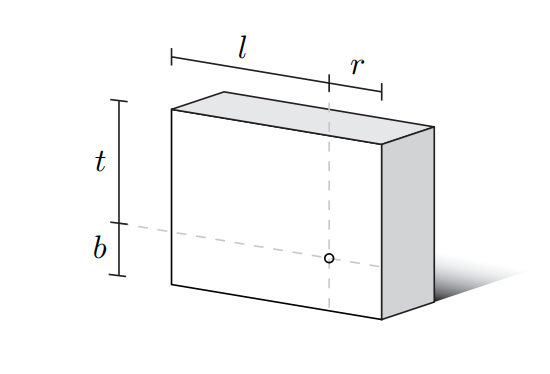
\includegraphics[width=0.7\textwidth]{figures/Preliminaries/off-axis.png}
    \caption{}\label{Off-axis projection}
\end{figure}

\clearpage
\part{Method and Experiment}

\section{Method}

To implemented the proposed system, we divide the system into three main parts: head tracking, 3D effect, and curved display corrention. In Section4.1, we introduce the basic structure of algorithm and the intra-process communication framework used. Section4.2 introduced head tracking part, which is responsible for tracking the user's head movement and providing the user head's position and do filter. Section4.4 introduce methods and details about how to implement 3D effect, including unity simulation part and off-axis projection implementation. Section4.4 introduce the curved display correction, which is responsible for correcting the image distortion on the curved display.

\subsection{Framework}
System's framework can be devided into two parts in platform level: C++ level and Unity level. C++ level is responsible for head tracking and image correction, and Unity level is responsible for off-axis projection and simulation constructing. The communication between C++ and Unity is based on Robot Operating System 2(ROS2)\cite{ros2} and Unity's ROS2 plugin\cite{ros2forunity}, since ros2 provided a convinience way to both communication and data visualization. Code structure is shown in Figure 12.

\begin{figure}[htb]
    \centering
    \includegraphics[width=0.5\textwidth]{example-image-a}
    \caption{code structure and working-flow}\label{F:test-a}
\end{figure}

In detector, we use YuNet\cite{Wu_2023} to detect the user's face and get the face's key points. Then keypoints is sent to pnp solver, which return head's position in camera frame and send to tracker. Tracker node process head's position, applying CV motion model to kalman filter and send result to Unity part. In Unity, we have constructed a simulation environment, which include two position-synchronized cameras. Camera1 to simulate the user's eye, and camera2 a virtual environment rendering camera. Once camera2 finish its rendering, result image will be sent to wrap node, which apply finally image correction and send to display.

\subsection{Head Tracking}
In head tracking part, we use YuNet\cite{Wu_2023} to detect the user's face and get the face's key points, and applying CV motion model to do filter.

\subsubsection{Detector and Locator}
OpenCV 4.5.4\cite{opencv_4_5_4} have integrated YuNet as one of face landmark detection function. Network structure of YuNet is shown in Figure 13. 

\begin{figure}[htb]
    \centering
    \includegraphics[width=0.5\textwidth]{example-image-a}
    \caption{YuNet network structure, while onnx model can be found at \href{https://github.com/opencv/opencv_zoo/tree/main/models/face_detection_yunet}{OpenCV Model Zoo}}\label{F:test-a}
\end{figure}

In OpenCV's API, YuNet accept a RGB image as input, and return a n * 14 size matrix, while n is the number of faces detected in the image. For each row, the first 4 elements are the bounding box of the face, and the rest 10 elements are the key points of the face, representing right eye, left eye, nose, right chin and left chin.

% For localization, OpenCV also privide solvePnP() as a pnp solve api. Since solvePnP() function return camera's pose in world frame, we defined face-frame pnp's world frame(Figure 14).



For localization, OpenCV also provide solvePnP() as a pnp
 solve api, with input of 3d points(world frame), 2d points(opencv's image frame), camera matrix and distortion matrix as input, output of camera's pose in world frame. Since solvePnP() function return camera's pose in world frame, world frame is defineded same as face-frame. Figure 14 shows the face-frame definition.

\begin{figure}[htb]
    \centering
    \includegraphics[width=0.5\textwidth]{example-image-a}
    \caption{Face-frame definition}\label{F:test-a}
\end{figure}

In addition, ePnP is chosen by its low-latency\cite{EPnP_2009}. Also, we've obtained camera's intrinsic matrix and distortion matrix by ros2 camera calibration package\cite{ros2_camera_calibration}, and applicated 3d-keypoints in a sample human head's model from Soheil M. etc(2023)'s work.\cite{soheil2023facial}

\subsubsection{Kalman Filter}
Consider the general movement of human head, we choose Kalman Filter as our motion model, since the head movement is a linear dynamic system. The state variables can be defined as head's:
\begin{equation}
    \begin{aligned}
        x_k &= \begin{bmatrix} x & y & z & v_x & v_y & v_z \end{bmatrix}^T
    \end{aligned}
\end{equation}
\begin{equation}
    \begin{aligned}
        z_k &= \begin{bmatrix} x & y & z \end{bmatrix}^T
    \end{aligned}
\end{equation}
while $x, y, z$ is the position of the head, and $v_x, v_y, v_z$ is the velocity of the head. 
Consider head's movement as a constant velocity(cv) model, the state transition equations can be defined as:
\begin{equation}
    \begin{cases}
        x' = x + v_{x} \cdot dt \\
        y' = y + v_{y} \cdot dt \\
        z' = z + v_{z} \cdot dt 
    \end{cases}
\end{equation}
and observation equations:
\begin{equation}
    \begin{cases}
        x_m = x \\
        y_m = y \\
        z_m = z
    \end{cases}
\end{equation}
while $x_m, y_m, z_m$ are variables in measurement space, and $dt$ is the time interval between two frames. 
.
In this case, we can generate the state transition matrix $F_k$ and measurement matrix $H_k$ as:

\begin {equation}
    F_k = \begin{bmatrix} 1 & 0 & 0 & dt & 0 & 0 \\ 0 & 1 & 0 & 0 & dt & 0 \\ 0 & 0 & 1 & 0 & 0 & dt \\ 0 & 0 & 0 & 1 & 0 & 0 \\ 0 & 0 & 0 & 0 & 1 & 0 \\ 0 & 0 & 0 & 0 & 0 & 1 \end{bmatrix} 
\end {equation}

\begin {equation}
    H_k = \begin{bmatrix} 1 & 0 & 0 & 0 & 0 & 0 \\ 0 & 1 & 0 & 0 & 0 & 0 \\ 0 & 0 & 1 & 0 & 0 & 0 \end{bmatrix}
\end {equation}

By given the process noise covariance matrix $Q_k$ and measurement noise covariance matrix $R_k$ a proper value, we can apply Kalman Filter to track the head's position.

\subsection{3D Effect}
\subsubsection{Off-axis Projection}

\subsubsection{Curved Displays Correction}



\section {Experiment}

\subsection{Measurement of Head Tracking}
\subsection{Algorithm speed}
\subsection{Illusion Effects}


\subsection{Curved Displays Correction}

\subsection {Experiment}



\part{Conclusion and Future Work}
\section{Conclusion}
\section{Future Work}

% % !Mode:: "TeX:UTF-8"
% !TEX program  = xelatex
% \section{免责声明}
% \begin{enumerate}[label={\alph*)}]
%     \item 本模板的发布遵守 \LaTeX\ Project Public License,使用前请认真阅读协议内容。
%     \item 南方科技大学教学工作部只提供毕业论文写作指南,不提供官方模板,也不会授权第三方模板为官方模板,所以此模板仅为写作指南的参考实现,不保证格式审查老师不提意见. 任何由于使用本模板而引起的论文格式审查问题均与本模板作者无关。
%     \item 任何个人或组织以本模板为基础进行修改,扩展而生成的新的专用模板,请严格遵守 \LaTeX\ Project Public License 协议。由于违犯协议而引起的任何纠纷争端均与本模板作者无关。
% \end{enumerate}
\section {Introduction}
Amid the brisk pace of technological evolution, Virtual Reality (VR) has emerged as a focal point due to its capacity to deliver immersive and interactive experiences. Traditional VR frameworks, however, have typically necessitated the use of specialized head-mounted displays (HMDs). This requirement not only circumscribes their practicality but also impacts user comfort and the viability of extended engagement. This report delineates an innovative approach to implementing glasses-free VR, aimed at severing the reliance on conventional HMDs through the adoption of monocular distance measurement and off-axis projection techniques, thus amplifying user accessibility and involvement.

The principal technological underpinnings of this project involve the extraction of facial  landmarks (executed via OpenCV), the determination of facial positions using PnP algorithms, and the employment of a Kalman filter to diminish the effects of keypoint jitter. Through off-axis projection, we successfully render scenes crafted in Unity in a manner that engenders a VR experience devoid of any requisite headgear.

This technology's ingenuity lies in its ability to surmount both the physical and fiscal impediments associated with standard VR modalities, while also facilitating a more organic and intuitive user interaction by meticulously tracking the user’s facial and eye movements. The prospective applications of this methodology are extensive, spanning entertainment and gaming to sectors like education, healthcare, and industrial design, offering an immersive digital milieu accessible without the dependency on supplementary apparatus.

% % !Mode:: "TeX:UTF-8"
% !TEX program  = xelatex
\section{Domestic and International Research Status}
% 文类的接口的命名均为汉字,意思为字面意思,如有疑问,欢迎在 GitHub 提出 \href{https://github.com/Iydon/sustechthesis/issues}{Issues}。
\lipsum[1]

\subsection{汉化字号接口}
本接口主要使用 \texttt{ctex} 宏包。

\verbbox{\初号},\verbbox{\小初},\verbbox{\一号},\verbbox{\小一},\verbbox{\二号},\verbbox{\小二},\verbbox{\三号},\verbbox{\小三},\verbbox{\四号},\verbbox{\小四},\verbbox{\五号},\verbbox{\小五},\verbbox{\六号},\verbbox{\小六},\verbbox{\七号},\verbbox{\八号}。


\subsection{汉化字体接口}
可能本机上部分字体不存在,导致部分字体无法使用。

\verbbox{\宋体},\verbbox{\黑体},\verbbox{\仿宋},\verbbox{\楷书},\verbbox{\隶书},\verbbox{\幼圆},\verbbox{\雅黑},\verbbox{\苹方}。


\subsection{字体效果接口}

建议在正文时使用 \verb|\textbf{}|,\verb|\textit{}| 调用\textbf{粗体}与\textit{斜体}。

It is recommended to use \verb|\textbf{}|,\verb|\textit{}| to call \textbf{Bold} and \textit{ItalicFont}.

\verbbox{\粗体},\verbbox{\斜体}。


\subsection{格式相关接口}
\subsubsection{命令}
例子请参考前文,在写论文初期,可以注释掉标题页等不必要信息,以加快编译速度。

\verbbox{\设置信息},\verbbox{\目录},\verbbox{\下划线},\verbbox{\中文标题页},\verbbox{\英文标题页},\verbbox{\中文诚信承诺书},\verbbox{\英文诚信承诺书},\verbbox{\摘要标题},\verbbox{\参考文献},\verbbox{\附录},\verbbox{\致谢}。

\subsubsection{环境}
摘要环境均需一个参数,为关键词:\verb|\begin{}{}...\end{}|。

\verbbox{中文摘要},\verbbox{英文摘要}。

% \input{sections/examples/details.tex}
% \input{sections/examples/figures.tex}
% \input{sections/examples/tutorial.tex}

\clearpage

\参考文献
  \printbibliography[heading=none]\clearpage
% \附录
%   \input{sections/examples/appendix.tex}\clearpage
% \致谢
%   \input{sections/examples/thanks.tex}
\end{document}

